%!TEX root = ../main.tex

\chapter[DAEs Index Reduction and Numerical Solution]{Differential-Algebraic Equations Index Reduction and Numerical Solution}
\label{chap6:daes}

\subsubsection{Copyright Notice}
Part of this chapter has been first published in
%
\begin{center}
  \begin{minipage}{0.9\textwidth}
    \fullcite{stocco2024symbolic}
  \end{minipage}
\end{center}
\begin{center}
  \begin{minipage}{0.9\textwidth}
    \fullcite{stocco2024matrix}
  \end{minipage}
\end{center}
%
by Springer and Elsevier, respectively. Reproduced with permission from Springer and Elsevier.

\begin{center}
  $\ast$~$\ast$~$\ast$
\end{center}

We present an algorithm for the index reduction of first-order differential-algebraic equations. The proposed approach can be applied to generic differential-algebraic equations and exploits neither a priori knowledge nor ad hoc techniques to leverage the specific formulation of the system. The index reduction is performed only by using symbolic manipulation and linear algebra techniques. It is based on the successive separation of the differential and algebraic equations of the system and the subsequent differentiation of the algebraic part. Improved symbolic matrix factorization is used to perform the differential-algebraic equations partitioning, ensure numerical stability, and limit the expression swell of the reduced-index system. The effectiveness of the algorithm is validated through symbolic-numerical examples on a wide range of systems, including physical systems, engineering applications, and ``artificial'' differential-algebraic equations with specific properties. The proposed symbolic index reduction algorithm is implemented in \Maple{} as part of an open-source library.

% % % % % % % % % % % % % % % % % % % % % % % % % % % % % % % % % % % % % % % %

\section{Introduction}
\label{chap6:sec:introduction}

\acp{DAE} are extensively used in dynamic system modeling. The challenge in numerically solving a \ac{DAE} system is assessed through its differentiation index, commonly referred to as ``the'' index~\cite{campbell1995index}. Achieving accurate simulations necessitates converting high-index \acp{DAE} into low-index counterparts, posing a well-recognized challenge~\cite{petzold1982differential}. This process involves transforming a \ac{DAE} system into an equivalent system with a lower index through successive differentiation of the system equations. For this reason, the differentiation index is roughly defined as the number of times algebraic equations are differentiated to obtain an equivalent system of \acp{ODE} with invariants. Index reduction is a crucial step prior to the numerical integration of \acp{DAE}, as integrating high-index systems can be impractical. The primary obstacle lies in the necessity to solve nonlinear systems of equations at each integration step, which can be computationally expensive and, in certain cases, numerically unstable. Specific numerical techniques, introduced in~\cite{petzold1982differential, thomsen1999numerical, baumgarte1972stabilization}, have been developed to address this challenge. However, these methods are not universally effective and may be inapplicable to some high-index \acp{DAE}. Consequently, index reduction becomes an indispensable preliminary stage before numerical integration~\cite{lamour2013differential}.

Given its complicated nature, index reduction has been the subject of extensive research and is often carried out by leveraging the specific formulation of the \ac{DAE} system, like in the multi-body modeling~\cite{zhou2005implicit, zhou2007symbolic, zhou2007symbolicseq, bayo1988modified, wehage1982generalized}. When the specific formulation of the \ac{DAE} system is not known a priori, or the system is not in a specific form, the index reduction process becomes more challenging. Many current simulation software packages for dynamic systems use index-reduction algorithms based on the \ac{SA} of the system, such as the Pantelides algorithm~\cite{pantelides1988consistent} and the dummy derivatives method~\cite{mattsson1993index}, which are subcases of the Pryce's $\Sigma$-method~\cite{pryce1998solving, pryce2001simple, nedialkov2007solvingI, nedialkov2007solvingII, nedialkov2008solvingIII, nedialkov2015algorithm, tan2016symbolic, mckenzie2017structural}. These algorithms are effective in reducing the index of most of the systems, but they can fail either for numerical cancellations~\cite{iwata2019index} or underestimation of the differentiation index~\cite{pantelides1988consistent, unger1995structural}, like in the case of Rei{\ss}ig's \acp{DAE} family~\cite{reissig2000differential}. Symbolic manipulation is proven to be successful in restating a \acp{DAE} on which the $\Sigma$-method fails to a \acp{DAE} on which the \ac{SA} may succeed~\cite{tan2016symbolic}.

Index reduction based on symbolic-numeric aided \ac{SA} has been successful in handling failures of the Pryce's $\Sigma$-method~\cite{tan2016symbolic} as well as in performing symbolically-informed \ac{SA}~\cite{chowdhry2004symbolic}. This latter \ac{SA} approach, which is named $\sigma v$-method, uses symbolic-numeric \ac{LU} factorization for variable substitution and rank determination on linear constant coefficient \acp{DAE}. A valuable attempt to use pure symbolic manipulation in \acp{DAE} index reduction is presented in~\cite{zhou2005implicit, zhou2007symbolic, zhou2007symbolicseq}, where implicit involutive form and \ac{LU} decomposition are successfully used to reduce the index of a simple constrained multi-body system. It is clear that index reduction algorithms based on pure symbolic matrix factorization represent a viable alternative to classic \ac{SA} techniques. However, symbolic matrix factorization feasibility is strongly tied to the performance of the symbolic computation kernel and its capabilities~\cite{zhou2008fraction}. Large expressions can lead to strong performance degradation of the kernel. Techniques aimed at limiting this decrease of performance while performing symbolic linear algebra operations are presented in~\cite{zhou2006hierarchical, zhou2007symbolic, zhou2007symbolicseq}. In these works, the hierarchical representation of expressions is applied to matrix factorization tasks. Nonetheless, the \LULEM{} package~\cite{carette2006linear}, which implements large expression management strategies in \ac{LU} decomposition, significantly outperforms the \Maple{}'s built-in matrix factorization routines.

Following this brief introduction of the most widely recognized index reduction algorithms, we provide an overview of the specific index reduction algorithms found in current state-of-the-art software. The following list is limited to the most prominent solutions dedicated to dynamic system modeling and simulation that are widely adopted in both academia and industry.
%
\begin{itemize}
  \setlength{\itemsep}{-0.2em}
  \item \Matlab{} uses the Pantelides algorithm~\cite{pantelides1988consistent} to reduce the \acp{DAE} to index-1. Alternatively, or if the latter fails, the more reliable but slower Gaussian elimination algorithm can be employed to obtain an index-0 \ac{DAE} system~\cite{matlab}.
  \item \textsc{Modelica}-based software~\cite{mattsson1997modelica, mattsson1998physical} and \textsc{ModelingToolkit}~\cite{modelingtoolkit} employ the Pantelides algorithm~\cite{pantelides1988consistent} along with the dummy derivatives method~\cite{mattsson1993index} to automatically perform the reduction to index-1 \acp{DAE}.
  \item \Mathematica{} offers a comprehensive suite of index reduction algorithms~\cite{mathematica}. It can reduce the index of \acp{DAE} using the Pantelides~\cite{pantelides1988consistent} or structural matrix~ \cite{unger1995structural, chowdhry2004symbolic} methods. Additionally, it implements dummy derivatives~\cite{mattsson1993index} and projection methods for taking hidden constraints into account during numerical integration.
  \item \Maple{} performs symbolic index reduction within the \texttt{dsolve} function~\cite{maple}. However, the implemented algorithms are not documented or referenced. They are likely to be based on the projection method outlined in~\cite{shmoylova2013simplification}. Notably, the patents by the same authors~\cite{postma2012exact, shmoylova2012method, postma2015exact} discuss techniques for eliminating isolated parameters, extracting parameter sub-expressions from \acp{DAE}, and establishing minimal disconnected clusters of parameter sub-expressions. We would like to point out that this information is to be taken with caution, as \Maple{} does not provide specific references on this topic.
\end{itemize}
%
All the showcased software solutions offer integrators for index-0 and index-1 \acp{DAE}. Depending on the system's stiffness, users can select the most appropriate algorithm for numerically integrating the reduced-index system.

The absence of user-invocable standalone functions within the \Maple{} environment that allows for the automatic index reduction of \acp{DAE}, and the inability to extract both the reduced-index system and invariants from the \texttt{dsolve} function, are the primary motivations of this research. Furthermore, recent advances in symbolic matrix factorization, combined with expressions hierarchical representation techniques, provide valuable tools that enable us to further investigate the applicability of a novel algorithm for the index reduction of \ac{DAE} systems, firstly presented in~\cite{stocco2024symbolic} as a preliminary work. The proposed methodology is similar to the previous work of~\citet{chowdhry2004symbolic} and extends it to generic first-order \acp{DAE}, linear in the states' derivatives. Nonetheless, the proposed algorithm does not work on the structural matrix of the system but on the \ac{DAE} system symbolic expressions. Specifically, the idea of using matrix factorization for variable substitution and rank determination is adopted to iteratively separate the differential and algebraic equations of the system. The algebraic equations are then differentiated to obtain an equivalent system with a lower differentiation index. Not less important, new libraries for symbolic matrix factorization (\LAST{}), large expression management (\LEM{}), and signature computation (\SIG{}) are presented. These libraries are based on the \LULEM{} package and extend the work of~\citet{zhou2006hierarchical, carette2006linear} and~\citet{zhou2007symbolic}. The newly presented libraries are designed to ensure the numerical stability of the numerically evaluated expressions, limit the expression swell, and provide an updated object-oriented interface. The effectiveness of the presented index reduction algorithm is validated through symbolic-numerical examples on a wide range of systems, including physical systems, engineering applications, as well as ``artificial'' systems with specific properties. The proposed algorithm is implemented in the \Maple{} environment and is available as a collection of open-source packages~\cite{last2023source,lem2023source}. Furthermore, the insights and the techniques presented in~\cite{zhou2006hierarchical, carette2006linear, zhou2007symbolic} are used to improve the presented algorithm to embed the hierarchical representation of expressions in a future implementation of the algorithm.

The manuscript is organized as follows. After this introduction (Section~\ref{chap6:sec:introduction}), the index reduction algorithm is presented in Section~\ref{chap6:sec:algorithm}. The expression swell mitigation, as well as the details on the symbolic matrix factorization, are discussed in Sections~\ref{chap6:sec:expression_swell} and \ref{chap6:sec:matrix_factorization}. The effectiveness of the algorithm is showcased through symbolic-numerical examples in Section~\ref{chap6:sec:examples}. Finally, Sections~\ref{chap6:sec:future_work} and~\ref{chap6:sec:conclusions} report future developments and conclusions respectively. In~\ref{chap6:sec:cokernel} details on cokernel computation are reported. The newly developed object-oriented symbolic linear algebra (\ref{chap6:sec:last}), large expression management (\ref{chap6:sec:lem}) and signature computation (\ref{chap6:sec:signature}) package descriptions are also included in the appendices. The symbolic index reduction algorithm is implemented in the \Maple{} language and is available as part of the open-source \Indigo{} library~\cite{indigo2023source}. Its usage is illustrated in~\ref{chap6:sec:index_reduction}. Notice that throughout the manuscript the \texttt{teletype} font indicates the use of \Maple{} and \Matlab{} commands or software implementations.

% % % % % % % % % % % % % % % % % % % % % % % % % % % % % % % % % % % % % % % %

\section{Index Reduction Algorithm}
\label{chap6:sec:algorithm}

In this section, we explore the theoretical aspect of reducing the differential index of \ac{DAE} systems. Specifically, to systematically reduce the \ac{DAE} system's index, a novel iterative algorithm is presented. This algorithm comprises two main phases: initially, the separation of the differential equations from the algebraic equations inherent in \acp{DAE}; and subsequently, the differentiation of the algebraic ones to obtain an equivalent system with a reduced index. The algorithm that is presented in this section is implemented in the \Maple{} environment and is available as an open-source package~\cite{indigo2023source}.

\subsection{Differential and Algebraic Equations Separation}
\label{chap6:sec:separation}

The initial phase of the index reduction procedure involves the partitioning of the \ac{DAE} system into its differential and algebraic equations. While in the case of small systems this can be accomplished through manual identification and isolation of the algebraic equations, this approach is inconvenient when dealing with large systems. An alternative method for automating the separation process leverages the cokernel, or left null space, of the \ac{DAE} system matrix, which is computed through matrix factorization techniques. The usage of the cokernel offers a more efficient and reliable means of accomplishing the separation task, variable substitution and not less importantly rank determination.

Consider a first-order system of \acp{DAE} $\mF$ of the form
%
\begin{equation}
  \label{chap6:eq:daes}
  \mF \overset{\mathrm{def}}{=}\mA \, \mxp - \mb = \m{0}.
\end{equation}
%
We denote the cokernel and its orthogonal complement of $\mA$ with $\mK$ and $\mN$ respectively (see~\ref{chap6:sec:cokernel} for details on the cokernel computation with symbolic matrix factorization). Notice that the cokernel is the subspace obtained by the span of $\mK$'s columns. For this reason, hereafter, we refer to the cokernel as the matrix $\mK$ whose columns span the cokernel. Using $\mK$ and $\mN$ it is possible to separate the algebraic part of the \acp{DAE}~\eqref{chap6:eq:daes} as
%
\begin{equation}
  \label{chap6:eq:separated_daes}
  \begin{cases}
    \mE \, \mxp = \mg \\[0.1em]
    \ma = \m{0}
  \end{cases} \text{,} \quad \text{where} \qquad \mA = \begin{bmatrix}
    \mE \\[0.2em]
    \m{0}
  \end{bmatrix} \text{,}
  \quad \text{and} \quad
  \mb = \begin{bmatrix} \mg \\[0.2em] \ma \end{bmatrix} \text{.}
\end{equation}
%
The separated equations of the \acp{DAE} are obtained by the left product of $\mK$ and $\mN$ as
%
\begin{equation}
  \begin{array}{l@{~}c@{~}l}
    \mE &=& \mN \, \mA \text{,} \\[0.1em]
    \mg &=& \mN \, \mb \text{,} \\[0.1em]
    \ma &=& \mK \, \mb \text{.}
  \end{array}
\end{equation}
%
This results in an equivalent \ac{DAE} system, where the algebraic equations $\ma$ are now explicit. The details of the cokernel and its orthogonal complement computation are discussed in~\ref{chap6:sec:cokernel}.

\subsection{Algebraic Equations Differentiation}
\label{chap6:sec:differentiation}

The algebraic equations in the \ac{DAE} system~\eqref{chap6:eq:separated_daes} are now differentiated as
%
\begin{equation}
  \label{chap6:eq:diff_daes}
  \dfrac{\mathrm{d}}{\mathrm{d}t} \ma = \mAd \, \mxp - \mgd \text{.}
\end{equation}
%
The \acp{DAE}~\eqref{chap6:eq:separated_daes} after differentiation of algebraic equations now take a form similar to that of~\eqref{chap6:eq:daes}, where
%
\begin{equation}
  \label{chap6:eq:reduced_daes}
  \mA = \begin{bmatrix} \mE \\[0.2em] \mAd\end{bmatrix} \text{,}
  \quad \text{and} \quad
  \mb = \begin{bmatrix} \mg \\[0.2em] \mgd\end{bmatrix} \text{.}
\end{equation}
%
The set of invariants, which are collected in $\mh$, is updated adding the algebraic equations $\ma$
%
\begin{equation}
  \mh \quad \xleftarrow[\text{update}]{\text{\, Invariants \,}} \quad \overset{{\text{The old $\mh$}}}{\begin{bmatrix} \overbrace{\mh} \\[0.2em] \ma \end{bmatrix}}.
\end{equation}
%
The iterative procedure, involving the sequential separation and differentiation of the algebraic segment of the system, is iterated until $\mA$ is non-singular. When $\mA$ is non-singular the \ac{DAE} corresponds to a system of \acp{ODE} compounded by the invariants $\mh$, which are the collection of the hidden constraints produced in the index reduction process. The invariants $\mh$ can be initialized empty or with user-defined algebraic equations aimed at preserving crucial system properties, such as energy conservation and/or momentum conservation. A pseudocode and a flowchart of the index reduction algorithm can be found in Algorithm~\ref{chap6:alg:index_reduction} and \figurename~\ref{chap6:fig:index_reduction}, respectively.

\begin{figure}[htp!]
  \centering
  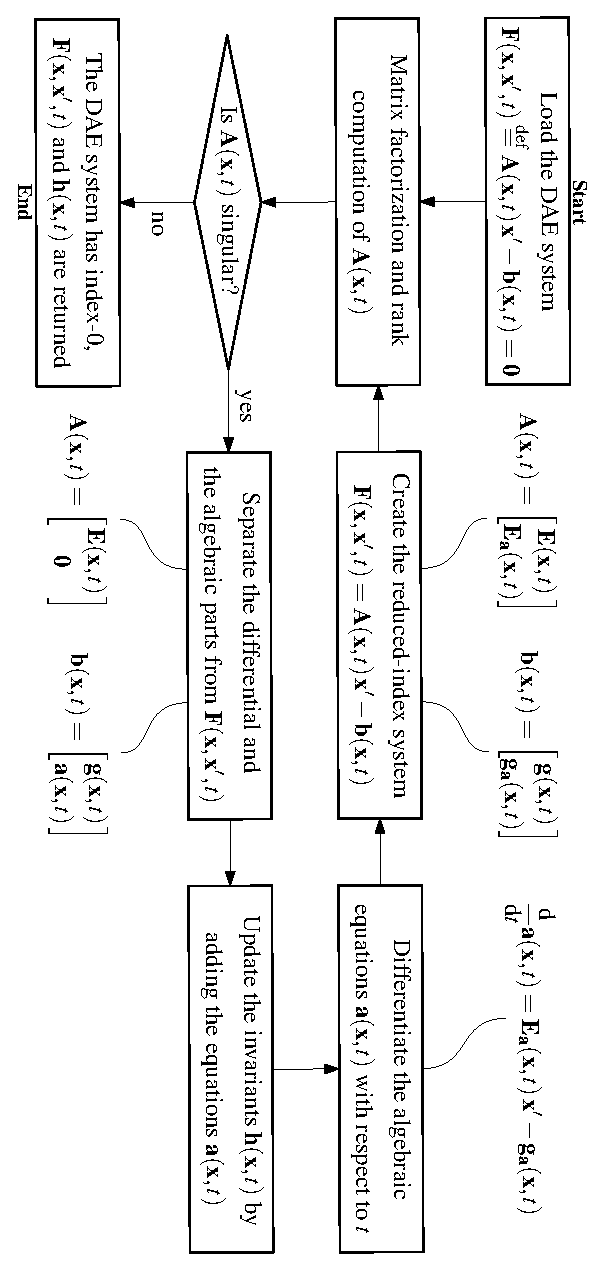
\includegraphics[angle=90, width=0.9\columnwidth]{flowchart}
  \caption{Flowchart of the index reduction algorithm.}
  \label{chap6:fig:index_reduction}
\end{figure}

\begin{algorithm}[H]
  \caption{Index reduction algorithm.}
  \label{chap6:alg:index_reduction}
  \begin{algorithmic}[1]
    \State \textbf{Require:} A \ac{DAE} system of the form $\mF \overset{\mathrm{def}}{=} \mA \, \mxp - \mb = \m{0}$.
    \Procedure{ReduceIndex}{$\mF$} \Comment{Index reduction procedure}
      \State $\mh \gets \varnothing$ \Comment{The set of invariants}
      \State $\mA, \, \mb \gets \mathrm{GenerateMatrix}(\mF, \, \mxp)$ \Comment{The \ac{DAE} system matrix}
      \State $m \gets \mathrm{Size}(\mx)$\Comment{The size of $\mx$}
      \While{$\mA$ is singular}
        \State $\displaystyle\triangleright$ Differential and algebraic equations separation (Section~\ref{chap6:sec:separation})
        \State $\mL, \, \mU, \, \mP, \, \mQ \gets \mathrm{MatrixFactorization}(\mA)$ \Comment{LU or FFLU decomposition of $\mA$}
        \State $r \gets \mathrm{Rank}(\mU)$ \Comment{The rank of $\mU$ is equal to the rank of $\mA$}
        \State $\mI_1 \gets \mathrm{IdentityMatrix}(r, \, r)$ \Comment{The upper identity matrix}
        \State $\mI_2 \gets \mathrm{IdentityMatrix}(m-r, \, m-r)$ \Comment{The lower identity matrix}
        \State $\mE \gets [\mI_1, \, \m{0}] \, \mU \, \mQ^\top$ \Comment{The reordered part of $\mA$}
        \State $\mg \gets [\mI_1, \, \m{0}] \, \mL^{-1} \, \mP \, \mb$ \Comment{The differential part of $\mb$}
        \State $\ma \gets [\m{0}, \, \mI_2] \, \mL^{-1} \, \mP \, \mb$ \Comment{The algebraic part of $\mb$}
        \State
        \State $\displaystyle\triangleright$ Algebraic equations differentiation (Section~\ref{chap6:sec:differentiation})
        \State $\mAd, \, \mgd \gets \mathrm{GenerateMatrix}(\mathrm{Diff}(\ma, \, t), \, \mxp)$ \Comment{Differentiate the equations $\ma$}
        \State $\mA \gets \begin{bmatrix} \mE \\ \mAd \end{bmatrix}$ \quad and \quad $\mb \gets \begin{bmatrix}\mg \\ \mgd \end{bmatrix}$
        \Comment{The new matrix $\mA$ and vector $\mb$}
        \State $\mh \gets \mh \cup \ma$ \Comment{Add the algebraic equations to the set of invariants}
      \EndWhile \\
      \Return $\mA, \, \mb, \, \mh$ \Comment{The \acp{DAE} reduced to an \ac{ODE} system with invariants}
    \EndProcedure
  \end{algorithmic}
\end{algorithm}

\subsection{A Step-by-Step Example}
\label{chap6:sec:step_by_step}

Within this Section, we present the step-by-step results of the index reduction algorithm. To do so we exploit a simple non-stiff index-3 problem found in \Wolfram{}~\Mathematica{} documentation~\cite{mathematica}. The initial value problem is defined as follows
%
\begin{equation}
  \label{chap6:eq:index_3}
  \mF = \begin{bmatrix}
    x^{\prime}_{2} - x_{1} - \cos(t) \\
    x^{\prime}_{3} - x_{2} - \sin(t) \\
    x_{3} - \cos(t)
  \end{bmatrix},
\end{equation}
%
with states $\mx = [x_{1}, \, x_{2}, \, x_{3}]^\top$ and initial conditions $\mx_{0} = [-1, \, 0, \, 1]^\top$. Notice that the analytical solution of this problem is $\mx_{exact} = [\sin(t) - 2\cos(t), \, 2\sin(t), \, \cos(t)]^\top$. The index reduction algorithm is applied to the \ac{DAE} system~\eqref{chap6:eq:index_3} and the step-by-step results for the matrices $\mE$, $\mg$, and $\ma$ are reported here below.
%
\begin{equation*}
  \begin{array}{l}
    \text{Index-3 \acp{DAE}:} \quad \mE = \begin{bmatrix} \,
      0 & 1 & 0 \\
      0 & 0 & 1
    \, \end{bmatrix}, \quad
    \mg = \begin{bmatrix} \,
      \sin(t) - x_{1} \\
      \sin(t) - x_{2}
    \, \end{bmatrix}, \quad\quad~~~\,
    \ma = \begin{bmatrix} \,
      \cos(t) - x_{3}
    \, \end{bmatrix}. \\[1.0em]
    %
    \text{Index-2 \acp{DAE}:} \quad \mE = \begin{bmatrix} \,
      0 & 1 & 0 \\
      0 & 0 & 1
    \, \end{bmatrix}, \quad
    \mg = \begin{bmatrix} \,
      \sin(t) - x_{1} \\
      \sin(t) - x_{2}
    \, \end{bmatrix}, \quad\quad~~~\,
    \ma = \begin{bmatrix} \,
      2\sin(t) - x_{2}
    \, \end{bmatrix}. \\[1.0em]
    %
    \text{Index-1 \acp{DAE}:} \quad \mE = \begin{bmatrix} \,
      0 & 0 & 1 \\
      0 & 1 & 0
    \, \end{bmatrix}, \quad
    \mg = \begin{bmatrix} \,
      \sin(t) - x_{2} \\
      \sin(t) - x_{1}
    \, \end{bmatrix}, \quad\quad~~~\,
    \ma = \begin{bmatrix} \,
      \sin(t) - 2\cos(t) - x_{1}
    \, \end{bmatrix}. \\[1.0em]
    %
    \text{Index-0 \acp{DAE}:} \quad \mE = \begin{bmatrix} \,
      0 & 0 & 1 \\
      0 & 1 & 0 \\
      1 & 0 & 0
    \, \end{bmatrix}, \quad
    \mg = \begin{bmatrix} \,
      \sin(t) - x_{2} \\
      \sin(t) - x_{1} \\
      2\sin(t) + \cos(t)
    \, \end{bmatrix}, \quad
    \ma = \varnothing.
  \end{array}
\end{equation*}
%
The final form of the system is an index-0 \acp{DAE} system is then
%
\begin{equation}
  \label{chap6:eq:index_3_reduced}
  \mF = \begin{bmatrix}
    x^{\prime}_{2} - x_{1} - \cos(t) \\
    x^{\prime}_{3} - x_{2} - \sin(t) \\
    x^{\prime}_{1} - \cos(t) - 2\sin(t)
  \end{bmatrix},
  %
  \quad \text{with invariants} \quad
  %
  \mh = \begin{bmatrix}
    \cos(t) - x_{3} \\
    2\sin(t) - x_{2} \\
    \sin(t) - 2\cos(t) - x_{1}
  \end{bmatrix}.
\end{equation}
%
%Although the just presented example is not so complex and relevant for a real validation of the algorithm, it is useful to demonstrate the step-by-step results of the index reduction algorithm. Furthermore, the expression complexities encountered throughout the index reduction algorithm applied to the Index-3 problem are reported below in \tablename{}~\ref{chap6:tab:complexity}.

\subsection{Known Issues}

While the algorithm just presented is relatively straightforward to implement, it does have two major sources of potential issues that are both determined by the technology used and the fundamental theory.
%
\begin{itemize}
    \item \emph{Expression complexity}. Symbolic manipulation often leads to a growth in expression complexity. For this reason, expression simplification may not always be feasible due to software limitations or excessive CPU time demands. Making the algorithm insensitive to expression swell is thus crucial to its effectiveness.
    \item \emph{Numerical stability of symbolic matrix factorization}. The description of the algorithm involves the manipulation of matrices and vectors with either symbolic or mixed symbolic-numeric entries. Ensuring that symbolic matrix factorization maintains numerical stability is a critical requirement of the algorithm. In the case of \ac{LU} decomposition, inadequate pivoting strategies can lead to the generation of singular matrices, which in turn can cause the algorithm to fail~\cite{zhou2005implicit, zhou2007symbolic, giesbrecht2014symbolic}.
\end{itemize}
%
These are the two main points that we acknowledge in the implementation of the algorithm. In the forthcoming sections, each of these matters is discussed in detail, with recommendations on techniques and open-source software solutions that are used to address them.

% % % % % % % % % % % % % % % % % % % % % % % % % % % % % % % % % % % % % % % %

\section{Expression Swell}
\label{chap6:sec:expression_swell}

Symbolic computation software, such as \Maple{}, is capable of handling relatively large symbolic expressions. However, the increase in complexity can significantly slow down the execution of the index reduction algorithm discussed earlier, resulting in unacceptably long CPU times. This phenomenon, known as expression swell, is a primary contributor to the degradation of performance in symbolic computation kernels. Expression swell can be categorized into two types: \emph{inherent} and \emph{intermediate}. The latter occurs when a calculation temporarily generates extensive expressions during intermediate steps, en route to a potentially more compact final result. To mitigate this issue, hierarchical representation techniques offer a solution~\cite{zhou2006hierarchical}. The core concept of this hierarchical representation is to conceal (or \emph{veil}) intricate expressions from the user by employing auxiliary variables referred to as \emph{veil variables} (or \emph{veils}) and reveal (or \emph{unveil}) them only when they become strictly necessary. As an expert reader may have noticed, expression swell is directly linked to expression complexity. Specifically, choosing the right balance between the maximum expression complexity and the number of veiling variables is crucial to prevent expression swell and concurrently avoid excessive veiling. To effectively gauge expression complexity, a metric is necessary, and various definitions are available. While previous works have relied on the \Maple{}'s \texttt{length} function, we adopt a different measure: the computational cost, which is determined through the \texttt{cost} function in the \texttt{codegen} package. This approach, as illustrated in the forthcoming examples, offers insensitivity to the number of characters used to represent the expression internally to the symbolic computation kernel, thus ensuring superior control over the final expression size.

\paragraph{Large Expression Management} Specific modules designed to perform large expression management tasks and help the user handle hierarchical representations have been developed and documented in prior research~\cite{carette2006linear, zhou2007symbolic}. Among these, the \Maple{} module \texttt{LargeExpressions} already fulfills this role effectively. However, we have observed some minor limitations within this module, primarily arising from its user interface choices rather than the core concept or the programming technique employed. Consequently, they have refined it into a new, object-oriented package known as \LEM{}~\cite{lem2023source}. This updated version remains adherent to the original but offers enhanced control and straightforward utilization of veil variables. Notably, the object-oriented aspect allows for the creation of multiple instances of \LEM{} objects, thereby ensuring a sharp separation between veil variables to prevent potential conflicts resulting from improper usage. Examples of expression complexity calculation and large expression management are reported in~\ref{chap6:sec:complexity} and~\ref{chap6:sec:lem} respectively.

% % % % % % % % % % % % % % % % % % % % % % % % % % % % % % % % % % % % % % % %

\section{Matrix Factorization}
\label{chap6:sec:matrix_factorization}

As previously mentioned, matrix factorization is a widely employed technique for addressing linear systems. There are several types of decompositions, each with distinct properties and characteristics. The \ac{LU} decomposition ranks among the most commonly used approaches. In the context of purely numerical matrices, the practice aligns well with the theoretical foundations of the algorithm. However, when dealing with matrices consisting of either symbolic or mixed symbolic-numeric entries, the situation becomes more intricate~\cite{zhou2007symbolic}. In exact symbolic linear algebra scenarios, the cost of each operation during factorization can vary due to uncontrolled expression swell~\cite{zhou2006hierarchical}. Furthermore, the presence of symbolic values hinders the guarantee of numerical stability. Consequently, a key objective is to derive an output format that retains the symbolic structure of the input matrix and ensures numerical stability.

\paragraph{Fill-In} After the \ac{LU} factorization of a sparse matrix $\m{A}$, it is common to observe that the joint non-zeroes pattern of $\m{L}$ and $\m{U}$ exhibit either equal or lower sparsity compared to the original non-zero pattern of $\m{A}$. This phenomenon, known as fill-in, increases the number of algebraic operations required for solving linear systems, thereby diminishing performance. To mitigate this issue, specific reordering algorithms can be applied to minimize the fill-in of the factorized matrix. These algorithms mainly include \emph{nested dissection}~\cite{george1973nested, lipton1979generalized} and \emph{minimum degree}~\cite{markowitz1957elimination, rose1970symmetric} techniques. In this work, the minimum degree algorithm is preferred due to its ease of implementation. Conversely, the nested dissection is not yet considered as it involves working on the system's graph to identify graph separators, which is a less straightforward process in the symbolic case.

\paragraph{Numerical Stability} A crucial concern is ensuring the numerical stability of the symbolic code generated by matrix factorization. This issue is closely tied to \emph{zero-} or \emph{identity-testing} within symbolic expressions. When simplifying an expression is not feasible, the most commonly adopted methods for zero-testing are the probabilistic ones, which rely on the \emph{DeMillo-Lipton-Schwarz-Zippel lemma}~\cite{demillo1978probabilistic, schwartz1980fast, zippel1979probabilistic}.
%
\begin{itemize}
    \item The utilization of \emph{signature functions} involves the verification of equivalent expressions within a multitude of sub-expressions, a process facilitated by \emph{hashing} techniques~\cite{gonnet1984determining, char1984design, gonnet1986results, monagan1994signature}. In \Maple{}, each expression is stored in the simplification table, employing its signature as a key. A unique feature of these signatures is that equivalent expressions share the same signature. It is important to note that not all expressions can have their signatures determined, such as trigonometric expressions, however, opportune coordinates change for signature computation routines can be applied (see~\ref{chap6:sec:signature}).
    %
    \item The \emph{Hybrid symbolic-numerical} or \emph{static pivoting approach} offers a means to validate the stability of symbolic code through random numerical evaluations~\cite{giesbrecht2014symbolic, li1998making}. While this approach may be computationally less efficient compared to the former method, it yields satisfactory results. In other words, the ``choice of pivots is numerically good at most numerical specializations'' as emphasized in~\cite{giesbrecht2014symbolic}.
\end{itemize}

Based on these observations, the \ac{LU} and \ac{FFLU} factorizations are preferred over the QR and \ac{GJ} factorizations, as the former two involve simpler operations, thereby mitigating the issue of expression swell. Additionally, employing the \ac{LU} factorization with a minimum degree pivoting strategy proves superior in reducing fill-in.

\subsection{Improved Symbolic Pivoting Strategy}

A crucial detail of any \ac{LU}-based decomposition, either numerical or symbolic, is the pivoting strategy. This strategy hinges on the two aforementioned considerations: the degrees of the elements within the system matrix and the actual complexity of the expressions. The elements in the system matrix are arranged in descending order of their degrees, and the pivot of the least complexity is chosen. Sometimes these two features are conflicting. In such cases, the prioritization of the pivot with the lowest degree is preferred. It is important to notice that pivots consisting of numerical values take precedence over those with symbolic values, primarily due to their inherent minimum expression complexity. Throughout the pivoting process, the utilization of signatures is also employed whenever possible to confirm the presence of null expressions without the need for simplification. To summarize, the main steps of the pivoting strategy are the following.
%
\begin{enumerate}
  \item The degree for each of the system matrix's entries is calculated.
  \item The pivots are sorted by degree and a permutation is generated.
  \item The pivots are iterated in the order of the permutation and a candidate pivot is selected at each step.
  \item The candidate pivot is checked for null expressions with the aid of signatures.
  \item If the candidate pivot signature is not null, the expression is simplified and their complexity is calculated.
  \item If the candidate pivot is numeric, its numerical value is calculated, otherwise, it is set to infinity.
  \item The candidate pivot with the lowest complexity or largest absolute numeric value is selected as the best pivot and returned.
\end{enumerate}
%
A detailed description of the developed symbolic pivoting strategy is presented in Algorithm~\ref{chap6:alg:pivoting_strategy}.

\begin{algorithm}[H]
  \caption{Symbolic Pivoting Strategy.}
  \label{chap6:alg:pivoting_strategy}
  \begin{algorithmic}[1]
    \State \textbf{Require:} A $n \times m$ matrix $\m{A}$.
    \State \phantom{\textbf{Require:}} The $k$-th pivoting stage.
    \Procedure{SymbolicPivoting}{$\m{A}$, $k$} \Comment{Symbolic pivoting procedure for the $k$-th pivot}
    \State $\m{d}^r, \, \m{d}^c \gets \text{ComputeDegrees}(\m{A})$ \Comment{Calculate the row and column degrees of $\m{A}$}
    \For{$i$ \textbf{from} $k$ \textbf{to} $n$} \Comment{Iterate over the rows}
      \For{$j$ \textbf{from} $k$ \textbf{to} $m$} \Comment{Iterate over the columns}
        \State $D_{ij} \gets \infty$ \Comment{Set the combined degree matrix to infinity}
        \IfThen{$A_{ij} \neq 0$}
        {$D_{ij} \gets d^r_{i} \, \max(0, \, d^c_j-1) + d^c_j \, \max(0, \, d^r_i-1)$} \Comment{Compute the combined degree}
      \EndFor
    \EndFor
    \State $\mathcal{P} \gets \text{Sort}(\m{D})$ \Comment{Find the permutation that sorts the pivots list by degree cost}
    \State $q, \, l \gets \, 0, \, 0$ \Comment{Initialize the temporary pivot row and column indices}
    \State $p, \, p_c, \, p_n \gets \infty, \, \infty, \, \infty$ \Comment{Initialize the temporary pivot value, complexity and numerical value}
    \For{\textbf{all} $(i, j)$ \textbf{in} $\mathcal{P}$} \Comment{Iterate on the permutation set}
      \IfThen{$p_c \neq \infty$ \textbf{and} $D_{ij} > D_{ql}$}{\textbf{break}} \Comment{No more good pivots to check}
      \State $t \gets A_{ij}$ \Comment{Get the pivot value}
      \IfThen{$\text{Signature}(t) = 0$}{\textbf{continue}} \Comment{Skip the next pivot}
      \State $t \gets \text{Simplify}(t)$ \Comment{Try to simplify the pivot expression}
      \State $t_c \gets \text{ExpressionComplexity}(t)$ \Comment{Calculate the computational complexity of the pivot}
      \State $t_n \gets \infty$ \Comment{Set the default numerical value of the pivot to infinity}
      \IfThen{$t$ is numeric}{$t_n \gets \max(1, \, \mathrm{abs}(t))$} \Comment{Set the numerical value of the pivot}
      \If{$t_c < p_c$ \textbf{or} ($t_c = p_c$ \textbf{and} $t_n > p_n$)} \Comment{If the pivot is better than the current one}
        \State $q, \, l \gets i, \, j$ \Comment{Update the best pivot row and column indices}
        \State $p, \, p_c, \, p_n \gets t, \, t_c, \, t_n$ \Comment{Update the best pivot value, complexity and numerical value}
      \EndIf
    \EndFor \\
    \Return $p, \, q, \, l$ \Comment{The $k$-th pivot and its position}
    \EndProcedure
  \end{algorithmic}
\end{algorithm}

\paragraph{Symbolic Linear Algebra} The considerations outlined above aid as the foundations for the \LAST{} package~\cite{last2023source}. Within this package, the pivoting process has been designed to address the critical considerations of expression swell and numerical stability as previously discussed. This toolkit, integrated into the \Maple{} environment, is dedicated to symbolic linear algebra tasks. It builds upon the original research outlined in~\cite{zhou2008fraction} and encompasses a collection of functionalities for symbolic full-pivoting \ac{LU}, \ac{FFLU}, QR, and \ac{GJ} factorizations. Importantly, the \LAST{} package is intended to be used in tandem with the previously presented \LEM{} package~\cite{lem2023source}, contributing to the mitigation of expression swell.

% % % % % % % % % % % % % % % % % % % % % % % % % % % % % % % % % % % % % % % %

\section{Symbolic-Numerical Examples}
\label{chap6:sec:examples}

In this section, we showcase examples of high-index \ac{DAE} systems, which range in a wide spectrum, encompassing physical systems, engineering applications, as well as ``artificial'' \ac{DAE} systems with specific properties. These examples are employed to demonstrate the capabilities of the proposed index reduction algorithm. In particular, the following test cases are presented.
%
\begin{enumerate}
  \item A non-stiff index-3 problem found in \Wolfram{}~\Mathematica{} documentation~\cite{mathematica}, already showcased in Section~\ref{chap6:sec:step_by_step}.
  \item An index-3 problem with analytical solution, which describes the motion of a particle in 3D~\cite{campbell1995constraint}.
  \item A moderately stiff car-axis problem of index-3 describing a simple model of a car axis riding over a bumpy road~\cite{lioen1998test, mazzia2008test}.
  \item A slightly stiff index-1 system of an eight-nodes transistor-amplifier~\cite{lioen1998test, mazzia2008test}.
  \item A stiff index-2 system of an electric ring modulator~\cite{lioen1998test, mazzia2008test}.
  \item A dimension 5 Rei{\ss}ig's family \ac{DAE} system of index-1~\cite{reissig2000differential}.
  \item An index-3 system that describes the space shuttle reentry problem~\cite{brenan1995numerical}.
  \item An index-5 \ac{DAE} system, which describes the motion of a robotic arm~\cite{pryce1998solving}.
  \item The $\mathrm{N}$-Pendula with: (a)~$\mathrm{N} = 2$ and index-5~\cite{pryce1998solving}; (b)~$\mathrm{N} = 3$ and index-7~\cite{nedialkov2008solvingIII}; and (c)~$\mathrm{N} = 4$ and index-9~\cite{nedialkov2008solvingIII}.
\end{enumerate}
%
Examples 1 and 2 are accurately showcased in Sections~\ref{chap6:sec:step_by_step} and~\ref{chap6:sec:numerical_integration}, respectively. In specific, the first example demonstrates the step-by-step results of the index reduction algorithm presented here, while the second is used to visualize the numerical integration results of the reduced-index system, as well as the good conditioning of both the symbolic matrix factorization and the numerical integration scheme. The remaining tests are presented more concisely, and the expressions' complexity met during the index reduction process for each test is reported in \tablename{}~\ref{chap6:tab:complexity} of Section~\ref{chap6:sec:daes_complexity}. Similarly, the numerical results of the reduced-index systems are reported in \tablename{}~\ref{chap6:tab:numerical_integration} of Section~\ref{chap6:sec:numerical_integration}.

\subsection{Expression Complexity of the Reduced-Index Systems}
\label{chap6:sec:daes_complexity}

To demonstrate the capabilities of the proposed index reduction algorithm, we first consider the examples from a symbolic computation perspective. In particular, we consider the computational cost of the expressions generated during the presented procedure. The compactness of the expressions generated during the index reduction algorithm is a crucial aspect, as it ensures that limited computational overhead is introduced in the numerical integration of the reduced-index system, as well as in the projection of the solution on the hidden constraints. For each reduction stage of the examples considered, the computational cost is reported in \tablename{}~\ref{chap6:tab:complexity}. Notice that the computational costs of expressions that could not be simplified by \Maple{} within \SI{100}{\second} of CPU time are reported with a $\star$ symbol preceding them. The tests are performed on a \SI{2.6}{\giga\hertz} 6-Core Intel\textsuperscript{\textregistered} Core\textsuperscript{\textregistered} i7 computer.

The presented algorithm can successfully reduce the index of all the example \ac{DAE} systems here considered. The computational cost of the expressions generated during the index reduction procedure is comparable to the original \ac{DAE} system in most of the tests. However, it is important to highlight that in examples 7, 8 and 9c some of the expressions generated during the index reduction procedure are significantly more complex than the original \ac{DAE} system. In these cases, the \Maple{} symbolic computation kernel is not able to perform the simplification within \SI{100}{\second} of CPU time and the raw expressions are kept in the following reduction steps. As a consequence, the computational cost inherently increases throughout the following reduction steps. The \ac{DAE} systems that are hard to simplify are those having a matrix $\mA$ that is strongly dependent on the state variables $\mx$ or equivalently that retains complicated divisions in the vector $\mb$. In these cases, the computational cost of the vector $\ma$ increases significantly due to successive and repeated differentiation and symbolic factorization. The trigonometric identities provided by Weierstra{\ss}~\eqref{chap6:eq:weierstrass} or~\eqref{chap6:eq:zhou} can be used to obtain polynomial expressions and improve the detection of symbolic eliminations (see~\ref{chap6:sec:signature}). However, the use of such trigonometric identities does not typically lead to a significant improvement in the computational cost of the expressions generated during the index reduction procedure as the polynomial expressions obtained are hard to simplify as well.

Another aspect that is important to mention is the sudden increase in computational complexity of the expressions generated in the last reduction step. Even if this increase is not critical to the correct index reduction as the presented algorithm is robust to expression swell, it does undermine the numerical efficiency of the final \ac{DAE} system. This highlights the need for further research on expression swell mitigation techniques in symbolic computation (see~\ref{chap6:sec:lem}), as well as the need to use integrators that can handle index-1 or even index-2 \acp{DAE}.

\setlength\tabcolsep{0.0pt}
\setlength{\LTcapwidth}{\textwidth}
{\footnotesize\centering\begin{longtable}{cccc}
  \caption[
    Expression complexity encountered throughout the index reduction algorithm of the test \ac{DAE} systems.
  ]{
    Expression complexity encountered throughout the index reduction algorithm of the test \ac{DAE} systems. \emph{Legend}: $\cf$ = functions, $\ca$ = additions, $\cm$ = multiplications, and $\cd$ = divisions. Expressions preceded by the $\star$ symbol could not be simplified within \SI{100}{\second} of CPU time in the \Maple{} environment.
  }
  \label{chap6:tab:complexity}
  \endfirsthead
  \endhead
  %
  \multicolumn{4}{c}{\textbf{1.~~Index-3 \acp{DAE}~\cite{mathematica}}} \\
  \toprule
  \textbf{Original \acp{DAE}} & \multicolumn{3}{c}{$\mF = 10\cf + 5\ca$ \quad $\mh = 0$} \\
  \midrule
  \textbf{Reduction step} & $\mE$ & $\mg$ & $\ma$ \\
  \midrule
  Index-3 \acp{DAE} & 0 & $4\cf + 2\ca$ & $2\cf + 1\ca$ \\
  Index-2 \acp{DAE} & 0 & $4\cf + 2\ca$ & $2\cf + 1\cm + 1\ca$ \\
  Index-1 \acp{DAE} & 0 & $4\cf + 2\ca$ & $3\cf + 1\cm + 1\ca$ \\
  Index-0 \acp{DAE} & 0 & $6\cf + 1\cm + 3\ca$ & $0$ \\
  \midrule
  \textbf{Reduced \acp{DAE}} & \multicolumn{3}{c}{$\mF = 12\cf + 1\cm + 6\ca$ \quad $\mh = 7\cf + 2\cm + 4\ca$} \\
  \bottomrule \\[-0.1em]
  %
  \multicolumn{4}{c}{\textbf{2.~~Particle Motion~\cite{campbell1995index}}} \\
  \toprule
  \textbf{Original \acp{DAE}} & \multicolumn{3}{c}{$\mF = 47\cf + 30\cm + 23\ca$ \quad $\mh = 0$} \\
  \midrule
  \textbf{Reduction step} & $\mE$ & $\mg$ & $\ma$ \\
  \midrule
  Index-3 \acp{DAE} & 0 & $39\cf + 36\cm + 13\ca$ & $7\cf + 10\cm + 6\ca$ \\
  Index-2 \acp{DAE} & 0 & $39\cf + 36\cm + 13\ca$ & $22\cf + 20\cm + 8\ca$ \\
  Index-1 \acp{DAE} & 0 & $39\cf + 36\cm + 13\ca$ & $68\cf + 72\cm + 33\ca$ \\
  Index-0 \acp{DAE} & $388\cf + 424\cm + 180\ca$ & $79\cf + 77\cm + 26\ca$ & 0 \\
  \midrule
  \textbf{Reduced \acp{DAE}} & \multicolumn{3}{c}{$\mF = 258\cf + 239\cm + 109\ca$ \quad $\mh = 97\cf + 102\cm + 47\ca$} \\
  \bottomrule \\[-0.1em]
  %
  \multicolumn{4}{c}{\textbf{3.~~Car-Axis~\cite{lioen1998test, mazzia2008test}} } \\
  \toprule
  \textbf{Original \acp{DAE}} & \multicolumn{3}{c}{$\mF = 108\cf + 131\cm + 56\ca$ \quad $\mh = 0$} \\
  \midrule
  \textbf{Reduction step} & $\mE$ & $\mg$ & $\ma$ \\
  \midrule
  Index-3 \acp{DAE} & $12\cm$ & $94\cf + 145\cm + 54\ca$ & $14\cf + 16\cm + 10\ca$ \\
  Index-2 \acp{DAE} & $12\cm$ & $94\cf + 145\cm + 54\ca$ & $26\cf + 45\cm + 15\ca$ \\
  Index-1 \acp{DAE} & $12\cm$ & $94\cf + 145\cm + 54\ca$ & $136\cf + 4\cd + 261\cm + 95\ca$ \\
  Index-0 \acp{DAE} & $1060\cf + 38\cd + 1901\cm + 717\ca$ & $431\cf + 8\cd + 842\cm + 268\ca$ & 0 \\
  \midrule
  \textbf{Reduced \acp{DAE}} & \multicolumn{3}{c}{$\mF = 896\cf + 4\cd + 1202\cm + 546\ca$ \quad $\mh = 176\cf + 4\cd + 322\cm + 120\ca$} \\
  \bottomrule \\[-0.1em]
  %
  \multicolumn{4}{c}{\textbf{4.~~Eight-Nodes Transistor-Amplifier~\cite{lioen1998test, mazzia2008test}}} \\
  \toprule
  \textbf{Original \acp{DAE}} & \multicolumn{3}{c}{$\mF = 55\cf + 21\cd + 29\cm + 41\ca$ \quad $\mh = 0$} \\
  \midrule
  \textbf{Reduction step} & $\mE$ & $\mg$ & $\ma$ \\
  \midrule
  Index-1 \acp{DAE} & $5\ca$ & $17\cf + 11\cd + 22\cm + 20\ca$ & $19\cf + 12\cd + 44\cm + 24\ca$ \\
  Index-0 \acp{DAE} & $24\cf + 26\cd + 24\cm + 24\ca$ & $18\cf + 12\cd + 26\cm + 20\ca$ & 0 \\
  \midrule
  \textbf{Reduced \acp{DAE}} & \multicolumn{3}{c}{$\mF = 74\cf + 26\cd + 87\cm + 49\ca$ \quad $\mh = 19\cf + 12\cd + 44\cm + 26\ca$} \\
  \bottomrule \\[-0.1em]
  %
  \multicolumn{4}{c}{\textbf{5.~~Electric Ring Modulator~\cite{lioen1998test, mazzia2008test}}} \\
  \toprule
  \textbf{Original \acp{DAE}} & \multicolumn{3}{c}{$\mF = 116\cf + 3\cd + 75\cm + 92\ca$ \quad $\mh = 0$} \\
  \midrule
  \textbf{Reduction step} & $\mE$ & $\mg$ & $\ma$ \\
  \midrule
  Index-2 \acp{DAE} & $0$ & $51\cf + 3\cd + 41\cm + 41\ca$ & $44\cf + 32\cm + 36\ca$ \\
  Index-1 \acp{DAE} & $86\cf + 68\cm + 66\ca$ & $262\cf + 13\cd + 416\cm + 220\ca$ & $10\cf + 2\cd + 18\cm + 11\ca$ \\
  Index-0 \acp{DAE} & $86\cf + 12\cd + 72\cm + 70\ca$ & $262\cf + 13\cd + 416\cm + 220\ca$ & 0 \\
  \midrule
  \textbf{Reduced \acp{DAE}} & \multicolumn{3}{c}{$\mF = 335\cf + 15\cd + 537\cm + 256\ca$ \quad $\mh = 54\cf + 2\cd + 50\cm + 47\ca$} \\
  \bottomrule \\[-0.1em]
  %
  \multicolumn{4}{c}{\textbf{6.~~Rei{\ss}ig's \acp{DAE}~\cite{reissig2000differential}}} \\
  \toprule
  \textbf{Original \acp{DAE}} & \multicolumn{3}{c}{$\mF = 13\cf + 26\ca$ \quad $\mh = 0$} \\
  \midrule
  \textbf{Reduction step} & $\mE$ & $\mg$ & $\ma$ \\
  \midrule
  Index-1 \acp{DAE} & $0$ & $4\cf + 2\ca$ & $10\cf + 5\ca$ \\
  Index-0 \acp{DAE} & $0$ & $14\cf + 5\ca$ & 0 \\
  \midrule
  \textbf{Reduced \acp{DAE}} & \multicolumn{3}{c}{$\mF = 32\cf + 13\ca$ \quad $\mh = 10\cf + 7\ca$} \\
  \bottomrule \\[-0.1em]
  %
  \multicolumn{4}{c}{\textbf{7.~~Space Shuttle Reentry~\cite{brenan1995numerical}}} \\
  \toprule
  \textbf{Original \acp{DAE}} & \multicolumn{3}{c}{$\mF = 116\cf + 16\cd + 77\cm + 38\ca$ \quad $\mh = 0$} \\
  \midrule
  \textbf{Reduction step} & $\mE$ & $\mg$ & $\ma$ \\
  \midrule
  Index-3 \acp{DAE} & $0$ & $112\cf + 13\cd + 247\cm + 49\ca$ & $6\cf + 1\cd + 30\cm + 11\ca$ \\
  Index-2 \acp{DAE} & $0$ & $112\cf + 13\cd + 247\cm + 49\ca$ & $66\cf + 2\cd + 529\cm + 123\ca$ \\
  Index-1 \acp{DAE} & $0$ & $112\cf + 13\cd + 247\cm + 49\ca$ & $903\cf + 4\cd + 8382\cm + 1369\ca$ \\
  Index-0 \acp{DAE} & $5612\cf + 28\cd + 50347\cm + 8204\ca$ & $112\cf + 13\cd + 247\cm + 49\ca$ & 0 \\
  \midrule
  \textbf{Reduced \acp{DAE}} & \multicolumn{3}{c}{$\star \mF = 5749\cf + 41\cd + 50599\cm + 8263\ca$ \quad $\mh = 975\cf + 7\cd + 8941\cm + 1503\ca$} \\
  \bottomrule \\[-0.1em]
  %
  \multicolumn{4}{c}{\textbf{8.~~Robotic Arm~\cite{pryce1998solving}}} \\
  \toprule
  \textbf{Original \acp{DAE}} & \multicolumn{3}{c}{$\mF = 125\cf + 19\cd + 56\cm + 64\ca$ \quad $\mh = 0$} \\
  \midrule
  \textbf{Reduction step} & $\mE$ & $\mg$ & $\ma$ \\
  \midrule
  Index-5 \acp{DAE} & $0$ & $66\cf + 3\cd + 50\cm + 35\ca$ & $16\cf + 12\ca$ \\
  Index-4 \acp{DAE} & $0$ & $66\cf + 3\cd + 50\cm + 35\ca$ & $24\cf + 6\cm + 14\ca$ \\
  Index-3 \acp{DAE} & $0$ & $66\cf + 3\cd + 50\cm + 35\ca$ & $162\cf + 2\cd + 138\cm + 114\ca$ \\
  Index-2 \acp{DAE} & $14\cf + 2\cd + 6\cm + 6\ca$ & $372\cf + 4\cd + 375\cm + 253\ca$ & $972\cf + 1\cd + 1062\cm + 770\ca$ \\
  Index-1 \acp{DAE} & $14\cf + 2\cd + 6\cm + 6\ca$ & $372\cf + 4\cd + 375\cm + 253\ca$ & $\star (6.5\cf + 5.6\cm + 1.8\ca)\cdot10^{6} + 4\cd$ \\
  Index-0 \acp{DAE} & $\star (8.3\cf + 7.1\cm + 2.3\ca)\cdot10^{7} + 58\cd$ & $(2.4\cf + 2.0\cm + 0.9\ca)\cdot10^{6} + 8\cd$ & 0 \\
  \midrule
  \textbf{Reduced \acp{DAE}} & \multicolumn{3}{c}{$\star \mF = (8.6\cf + 7.3\cm + 2.4\ca)\cdot10^{7} + 66\cd$ \quad $\star \mh = (6.5\cf + 5.6\cm + 1.8\ca)\cdot10^{6} + 7\cd$} \\
  \bottomrule \\[-0.1em]
  %
  \multicolumn{4}{c}{\textbf{9a.~~2-Pendula~\cite{pryce1998solving}}} \\
  \toprule
  \textbf{Original \acp{DAE}} & \multicolumn{3}{c}{$\mF = 67\cf + 31\cm + 31\ca$ \quad $\mh = 0$} \\
  \midrule
  \textbf{Reduction step} & $\mE$ & $\mg$ & $\ma$ \\
  \midrule
  Index-5 \acp{DAE} & $0$                  & $12\cf + 8\cm + 2\ca$ & $6\cf + 12\cm + 6\ca$ \\
  Index-4 \acp{DAE} & $1\cf + 5\cm + 1\ca$ & $16\cf + 12\cm + 3\ca$ & $4\cf + 4\cm + 1\ca$ \\
  Index-3 \acp{DAE} & $1\cf + 5\cm + 1\ca$ & $16\cf + 12\cm + 3\ca$ & $7\cf + 12\cm + 4\ca$ \\
  Index-2 \acp{DAE} & $1\cf + 5\cm + 1\ca$ & $16\cf + 12\cm + 3\ca$ & $18\cf + 2\cd + 30\cm + 9\ca$ \\
  Index-1 \acp{DAE} & $1\cf + 5\cm + 1\ca$ & $16\cf + 12\cm + 3\ca$ & $118\cf + 2\cd + 283\cm + 72\ca$ \\
  Index-0 \acp{DAE} & $555\cf + 21\cd + 1213\cm + 287\ca$ & $16\cf + 12\cm + 3\ca$ & $0$ \\
  \midrule
  \textbf{Reduced \acp{DAE}} & \multicolumn{3}{c}{
  $\mF = 482\cf + 2\cd + 807\cm + 229\ca$ \quad $\mh = 153\cf + 4\cd + 341\cm + 92\ca$} \\
  \bottomrule \\[-0.1em]
  %
  \multicolumn{4}{c}{\textbf{9b.~~3-Pendula~\cite{nedialkov2008solvingIII}}} \\
  \toprule
  \textbf{Original \acp{DAE}} & \multicolumn{3}{c}{$\mF = 67\cf + 31\cm + 31\ca$ \quad $\mh = 0$} \\
  \midrule
  \textbf{Reduction step} & $\mE$ & $\mg$ & $\ma$ \\
  \midrule
  Index-7 \acp{DAE} & $0$                   & $18\cf + 12\cm + 3\ca$ & $10\cf + 21\cm + 10\ca$ \\
  Index-6 \acp{DAE} & $2\cf + 10\cm + 2\ca$ & $26\cf + 20\cm + 5\ca$ & $4\cf + 4\cm + 1\ca$ \\
  Index-5 \acp{DAE} & $2\cf + 10\cm + 2\ca$ & $26\cf + 20\cm + 5\ca$ & $4\cf + 12\cm + 7\ca$ \\
  Index-4 \acp{DAE} & $2\cf + 10\cm + 2\ca$ & $26\cf + 20\cm + 5\ca$ & $18\cf + 2\cd + 30\cm + 9\ca$ \\
  Index-3 \acp{DAE} & $2\cf + 10\cm + 2\ca$ & $26\cf + 20\cm + 5\ca$ & $118\cf + 2\cd + 283\cm + 72\ca$ \\
  Index-2 \acp{DAE} & $2\cf + 10\cm + 2\ca$ & $26\cf + 20\cm + 5\ca$ & $992\cf + 3\cd + 2077\cm + 479\ca$ \\
  Index-1 \acp{DAE} & $2\cf + 10\cm + 2\ca$ & $26\cf + 20\cm + 5\ca$ & $6824\cf + 3\cd + 17665\cm + 4030\ca$ \\
  Index-0 \acp{DAE} & $54152\cf + 51\cd + 136388\cm + 28945\ca$ & $26\cf + 20\cm + 5\ca$ & $0$ \\
  \midrule
  \textbf{Reduced \acp{DAE}} & \multicolumn{3}{c}{
  $\mF = 28319\cf + 3\cd + 64295\cm + 15806\ca$ \quad $\mh = 7973\cf + 10\cd + 20092\cm + 4605\ca$} \\
  \bottomrule \\[-0.1em]
  %
  \multicolumn{4}{c}{\textbf{9c.~~4-Pendula~\cite{nedialkov2008solvingIII}}} \\
  \toprule
  \textbf{Original \acp{DAE}} & \multicolumn{3}{c}{$\mF = 67\cf + 31\cm + 31\ca$ \quad $\mh = 0$} \\
  \midrule
  \textbf{Reduction step} & $\mE$ & $\mg$ & $\ma$ \\
  \midrule
  Index-9 \acp{DAE} & $0$                   & $24\cf + 16\cm + 4\ca$ & $14\cf + 30\cm + 14\ca$ \\
  Index-8 \acp{DAE} & $3\cf + 15\cm + 3\ca$ & $36\cf + 28\cm + 7\ca$ & $4\cf + 4\cm + 1\ca$ \\
  Index-7 \acp{DAE} & $3\cf + 15\cm + 3\ca$ & $36\cf + 28\cm + 7\ca$ & $7\cf + 12\cm + 4\ca$ \\
  Index-6 \acp{DAE} & $3\cf + 15\cm + 3\ca$ & $36\cf + 28\cm + 7\ca$ & $18\cf + 2\cd + 30\cm + 9\ca$ \\
  Index-5 \acp{DAE} & $3\cf + 15\cm + 3\ca$ & $36\cf + 28\cm + 7\ca$ & $118\cf + 2\cd + 283\cm + 72\ca$ \\
  Index-4 \acp{DAE} & $3\cf + 15\cm + 3\ca$ & $36\cf + 28\cm + 7\ca$ & $992\cf + 3\cd + 2077\cm + 479\ca$ \\
  Index-3 \acp{DAE} & $3\cf + 15\cm + 3\ca$ & $36\cf + 28\cm + 7\ca$ & $6824\cf + 3\cd + 17665\cm + 4030\ca$ \\
  Index-2 \acp{DAE} & $3\cf + 15\cm + 3\ca$ & $36\cf + 28\cm + 7\ca$ & $(4.8\cf + 4\cd + 11.9\cm + 2.7\ca)\cdot10^{5}$ \\
  Index-1 \acp{DAE} & $3\cf + 15\cm + 3\ca$ & $36\cf + 28\cm + 7\ca$ & $\star (3.0\cf + 14.9\cm + 0.4\ca)\cdot10^{6} + 4\cd$ \\
  Index-0 \acp{DAE} & $\star (3.0\cf + 14.7\cm + 0.4\ca)\cdot10^{7} + 92\cd$ & $7\cf + 28\cm + 36\ca$ & 0 \\
  \midrule
  \textbf{Reduced \acp{DAE}} & \multicolumn{3}{c}{
  $\star \mF = (3.0\cf + 14.7\cm + 0.4\ca)\cdot10^{7} + 92\cd$ \quad $\star \mh = (3.1\cf + 15.1\cm + 0.5\ca)\cdot10^{6} + 18\cd$} \\
  \bottomrule
  %
\end{longtable}}

\subsection{Numerical Integration of the Reduced-Index System}
\label{chap6:sec:numerical_integration}

To demonstrate the numerical stability of the reduced-index system, we consider the second example, which is an index-3 problem with an analytical solution, taken from~\cite{campbell1995constraint}. It describes the motion of a particle inside a 3D torus surface. This system has three position variables $[x_{1}, \, x_{2}, \, x_{3}]^\top$, three velocity variables $[u_{1}, \, u_{2}, \, u_{3}]^\top$, and one constraint with Lagrange multiplier $\lambda$. The solution manifold is 4D, and the exact solution is
%
\begin{equation}
  \label{chap6:eq:torus_solution}
  \mx_{exact} = \begin{bmatrix}
    x_{1} \\ x_{2} \\ x_{3}
  \end{bmatrix} = \begin{bmatrix}
    (\rho \cos(2\pi - t) + r) \cos(t) \\
    (\rho \cos(2\pi - t) + r) \sin(t) \\
    \rho \sin(2\pi - t)
  \end{bmatrix}.
\end{equation}
%
The initial value problem is defined as follows
%
\begin{equation}
  \label{chap6:eq:torus}
  \mF = \begin{bmatrix}
    x^{\prime}_{1} - u_{1} \\
    x^{\prime}_{2} - u_{2} \\
    x^{\prime}_{3} - u_{3} \\
    u^{\prime}_{1} - u_{3}\cos(t) + x_{3}\sin(t) + u_{2} - 2 c x_{1}\lambda \\
    u^{\prime}_{2} - u_{3}\sin(t) - x_{3}\cos(t) - u_{1} - 2 c x_{2}\lambda \\
    u^{\prime}_{3} + x_{3} - 2x_{3}\lambda \\
    x_{1}^2 + x_{2}^2 + x_{3}^2 - 2r(x_{1}^2 + x_{2}^2)^{1/2} + r^2 - \rho^2
  \end{bmatrix},
\end{equation}
%
with $c = 1 - {r} / {(x_{1}^2 + x_{2}^2)^{1/2}}$, states $\mx = [x_{1}, \, x_{2}, \, x_{3}, \, u_{1}, \, u_{2}, \, u_{3}, \, \lambda]^{\top}$, initial conditions $\mx_{0} = [15, \, 0, \, 0, \, 0, \, 15, \, -5, \, \lambda]^{\top}$, and parameters $\rho = 5$ and $r = 10$. The index reduction algorithm is applied to the \ac{DAE} system and reduced to index-0. The expressions' complexity of the step-by-step results are reported in \tablename{}~\ref{chap6:tab:complexity}.

The numerical integration of the reduced-index system is performed through Implicit Euler, RadauIIA3, and RadauIIA5 Runge-Kutta methods. To respect the invariants during the integration the \emph{standard projection} method is applied \cite{hairer2000symmetric}. This method consists of projecting the solution $\mx$ of the numerically integrated system onto the invariants on the hidden constraints $\mh = \m{0}$, which is equivalent to the constrained minimization
%
\begin{equation}
  \underset{\tilde{\mx}}{\textrm{minimize}} \quad \dfrac{1}{2}\left(\mx - \tilde{\mx}\right)^2
    \quad \textrm{subject to} \quad
    \mh = \m{0}.
\end{equation}
%
To verify that the projection is performed correctly and does not affect the order of the Runge-Kutta method, numerical integration is performed in the interval $t \in [0, \, 2\pi]$ seconds with different integration time steps $\Delta t$. The error of the numerical integration $\varepsilon = \| \, \mx - \mx_{exact} \, \|_{\infty}$ is reported in \figurename~\ref{chap6:fig:torus_order}. As can be seen, the implemented projection preserves the order of the method for all the integration time steps. It is important to highlight that to obtain such results the absolute error tolerances of the integrator and the projection are both set to $\varepsilon = 10^{-10}$. The same tolerances are used in the numerical integration of the reduced-index system in the interval $t \in [0, \, 400\pi]$ seconds with step $\Delta t = 0.025$ seconds. The results are reported in \figurename~\ref{chap6:fig:torus_integration}, where Implicit Euler, RadauIIA3, and RadauIIA5 Runge-Kutta methods are employed, and the projection on the hidden constraints $\mh$ is performed. The effect of the projection is highlighted on the bottom left plot.

\begin{figure}[htp!]
  \centering
  \includetikz{./figures/chapter_6/torus_order.tex}
  \includetikz{./figures/chapter_6/torus_hidden.tex}
  \caption{Numerical integration error $\varepsilon = \| \, \mx - \mx_{exact} \, \|_{\infty}$ of the \acp{DAE}~\eqref{chap6:eq:torus} over different integration time steps $\Delta t$, along with the computed order of the method (left). The projection on the hidden constraints is performed and the invariants violation $\| \, \mh \, \|_{\infty}$ is reported (right). Notice that the implemented projection preserves the order of the method for all the integration time steps. The tests are performed in the interval $t \in [0, \, 2\pi]$ seconds, using Implicit Euler, RadauIIA3, and RadauIIA5 Runge-Kutta methods.}
  \label{chap6:fig:torus_order}
\end{figure}

\begin{figure}[htp!]
  \centering
  \includetikz{./figures/chapter_6/torus_implicit_euler.tex}
  \includetikz{./figures/chapter_6/torus_radauiia3.tex}
  \includetikz{./figures/chapter_6/torus_radauiia5.tex}
  \includetikz{./figures/chapter_6/torus_radauiia5_noproj.tex}
  \caption{Numerically integrated solution of the \acp{DAE}~\eqref{chap6:eq:torus} in the interval $t \in [0, \, 400\pi]$ seconds, with step $\Delta t = 0.025$ seconds, using Implicit Euler (top left), RadauIIA3 (top right), and RadauIIA5 (bottom left and right) Runge-Kutta methods. The first three plots show the numerical integration of the reduced-index system with projection on the hidden constraints $\mh$ produced by the index reduction algorithm. On the bottom right plot, the numerical integration of the reduced-index system is performed without projection on the manifold $\mh$ and substantial drift is observed.}
  \label{chap6:fig:torus_integration}
\end{figure}

The numerical integration for the remaining examples is also carried out, with outcomes detailed in \tablename{}~\ref{chap6:tab:numerical_integration}. This table reports the performance comparison between the joint index reduction algorithm and numerical integration schemes offered by \Maple{} and those of \Indigo{}. To ensure a fair comparison, both \Maple{} and \Indigo{} utilize the Runge-Kutta-Fehlberg 4(5) method for numerical integration of the \ac{DAE} system. Identical error tolerances are applied, with a relative tolerance of $10^{-6}$ and an absolute tolerance of $10^{-7}$. The results illustrate that the \Indigo{}'s index reduction algorithm implementation effectively generates numerically stable reduced-index \acp{DAE}, ensuring consistent integration across examples. However, exceptions arise in examples 8, 9b, and 9c. In example 8, \Maple{} fails to generate code for the reduced-index system within the expected time frame, thus the integration is not performed. This is due to the complexity of the expressions generated during the index reduction procedure, which overloads the \Maple{}'s \texttt{CodeGeneration} package.
Conversely, in examples 9b and 9c the integration of the reduced-index system is successfully performed using the non-default implicit RadauIIA5 method. Nonetheless, \Maple{}'s \texttt{dsolve} exceeded the function evaluations limit during the numerical integration of example 4 and fails in examples 5, 7, 8, 9b, and 9c due to either system's stiffness or high index.

It is important to highlight that during the numerical integration, the symbolic code is not regenerated by updating the index reduction. Therefore, for some numerical values of states and parameters, the \acp{DAE} system structure may change, leading to numerical instability. While this does pose a potential issue, it is worth noting that we have not encountered instability in the integration process, proving that the presented pivoting strategy is effective.

\setlength\tabcolsep{2.5pt}
\setlength{\LTcapwidth}{\textwidth}
{\footnotesize\centering\begin{longtable}{lccl}
  \caption{Numerical integration results of the reduced-index \ac{DAE} systems. The table reports the name and reference of the \ac{DAE} system, the index of the system, the integration interval $t \in [t_{\text{ini}}, \, t_{\text{end}}]$, and the outcomes of the whole code generation and integration process for both \Maple{} and \Indigo{}. If not otherwise specified, the tests are integrated using a Runge-Kutta-Fehlberg 4(5) method with a relative tolerance of $10^{-6}$ and an absolute tolerance of $10^{-7}$. The computation time limit is \SI{1000}{\second}, to both generate the necessary code and perform numerical computations. \emph{Legend:} \mycheckmark{} successful code generation and numerical integration, \mycrossmark{} errors in the code generation, numerical integration or time expired, and \mywarnmark{} warnings encountered or non-default settings used in the code generation or numerical integration.}
  \label{chap6:tab:numerical_integration}
  \endfirsthead
  \endhead
  %
  \toprule
  \textbf{Integrated \ac{DAE} system} &
  \multicolumn{3}{l}{\textbf{Integration outcomes and errors}} \\
  \midrule
  \multirow{1}{*}{\textbf{1.~~Index-3 \acp{DAE}~\cite{mathematica}}}
    & \Maple{}  & \mycheckmark{}\phantom{\mywarnmark{}} & Success \\ \cmidrule(l{4pt}){2-4}
    Index-3 \quad $t \in [0, 200\pi]$ seconds & \Indigo{} & \mycheckmark{}\phantom{\mywarnmark{}} & Success \\ \midrule
  \multirow{1}{*}{\textbf{2.~~Particle Motion~\cite{campbell1995index}}}
    & \Maple{}  & \mycheckmark{}\phantom{\mywarnmark{}} & Success \\ \cmidrule(l{4pt}){2-4}
    Index-3 \quad $t \in [0, 400\pi]$ seconds & \Indigo{} & \mycheckmark{}\phantom{\mywarnmark{}} & Success \\ \midrule
  \multirow{1}{*}{\textbf{3.~~Car-Axis~\cite{lioen1998test, mazzia2008test}}}
    & \Maple{}  & \mycheckmark{}\phantom{\mywarnmark{}} & Success \\ \cmidrule(l{4pt}){2-4}
    Index-3 \quad $t \in [0, 3]$ seconds & \Indigo{} & \mycheckmark{}\phantom{\mywarnmark{}} & Success \\ \midrule
  \multirow{1}{*}{\textbf{4.~~Eight-Nodes Transistor-Amplifier~\cite{lioen1998test, mazzia2008test}}}
    & \Maple{}  & \mycheckmark{}\mywarnmark{} & Warning, function evaluations limit exceeded \\ \cmidrule(l{4pt}){2-4}
    Index-1 \quad $t \in [0, 0.2]$ seconds & \Indigo{} & \mycheckmark{}\phantom{\mywarnmark{}} & Success \\ \midrule
  \multirow{1}{*}{\textbf{5.~~Electric Ring Modulator~\cite{lioen1998test, mazzia2008test}}}
    & \Maple{}  & \mycrossmark{}\phantom{\mywarnmark{}} & Error, time expired (in \texttt{dsolve}) \\ \cmidrule(l{4pt}){2-4}
    Index-2 \quad $t \in [0, 1]$ milliseconds & \Indigo{} & \mycheckmark{}\phantom{\mywarnmark{}} & Success \\ \midrule
  \multirow{1}{*}{\textbf{6.~~Rei{\ss}ig's \acp{DAE}~\cite{reissig2000differential}}}
    & \Maple{}  & \mycheckmark{}\phantom{\mywarnmark{}} & Success \\ \cmidrule(l{4pt}){2-4}
    Index-1 \quad $t \in [0, 10]$ seconds & \Indigo{} & \mycheckmark{}\phantom{\mywarnmark{}} & Success \\ \midrule
  \multirow{1}{*}{\textbf{7.~~Space Shuttle Reentry~\cite{brenan1995numerical}}}
    & \Maple{}  & \mycrossmark{}\phantom{\mywarnmark{}} & Error, time expired (in \texttt{dsolve}) \\ \cmidrule(l{4pt}){2-4}
    Index-3 \quad $t \in [332.8, 419.8]$ seconds & \Indigo{} & \mycheckmark{}\phantom{\mywarnmark{}} & Success \\ \midrule
  \multirow{1}{*}{\textbf{8.~~Robotic Arm~\cite{pryce1998solving}}}
    & \Maple{}  & \mycrossmark{}\phantom{\mywarnmark{}} & Error, time expired (in \texttt{dsolve}) \\ \cmidrule(l{4pt}){2-4}
    Index-5 \quad $t \in [0, 2]$ seconds & \Indigo{} & \mycrossmark{}\phantom{\mywarnmark{}} & Error, time expired (in \texttt{CodeGeneration}) \\ \midrule
  \multirow{1}{*}{\textbf{9a.~~2-Pendula~\cite{pryce1998solving}}}
    & \Maple{}  & \mycheckmark{}\phantom{\mywarnmark{}} & Success \\ \cmidrule(l{4pt}){2-4}
    Index-5 \quad $t \in [0, 60]$ seconds & \Indigo{} & \mycheckmark{}\phantom{\mywarnmark{}} & Success \\ \midrule
  \multirow{1}{*}{\textbf{9b.~~3-Pendula~\cite{nedialkov2008solvingIII}}}
    & \Maple{}  & \mycrossmark{}\phantom{\mywarnmark{}} & Error, time expired (in \texttt{dsolve}) \\ \cmidrule(l{4pt}){2-4}
    Index-7 \quad $t \in [0, 60]$ seconds & \Indigo{} & \mycheckmark{}\mywarnmark{} & Success with RadauIIA5 method \\ \midrule
  \multirow{1}{*}{\textbf{9c.~~4-Pendula~\cite{nedialkov2008solvingIII}}}
    & \Maple{}  & \mycrossmark{}\phantom{\mywarnmark{}} & Error, time expired (in \texttt{dsolve}) \\ \cmidrule(l{4pt}){2-4}
    Index-9 \quad $t \in [0, 60]$ seconds & \Indigo{} & \mycheckmark{}\mywarnmark{} & Success with RadauIIA5 method \\
  \bottomrule
  %
\end{longtable}}

% % % % % % % % % % % % % % % % % % % % % % % % % % % % % % % % % % % % % % % %

\section{Future Work}
\label{chap6:sec:future_work}

Despite its proven effectiveness, the presented symbolic index reduction algorithm offers scope for various methodological and implementation enhancements, which will be the subject of future research.

\subsection{Improved Pivoting Strategy}

Notably, the symbolic factorization relies on full-pivoting \ac{LU} decomposition. The choice of a pivot strategy holds paramount importance for achieving numerical stability in the reduced-index system. The present implementation selects pivots based on the minimum degree technique and expression complexity to minimize fill-in. However, this metric may not always be effective and the use of nested dissection or other techniques may further reduce fill-in and improve the numerical stability of the solution as well as the overall memory performance of the algorithm.

\subsection{Continued Symbolic Matrix Factorization}

In the present version, the matrix decomposition is repeated throughout the all \ac{DAE} system at every reduction step. This can be avoided by saving the partial factorization of the matrix $\mA$ and continuing it in the following reduction steps. This will significantly reduce the computational cost of the algorithm as only the newly differentiated expressions~\eqref{chap6:eq:diff_daes} need to be factorized at each iteration. This improvement would certainly improve the overall computational efficiency of the symbolic index reduction algorithm as the factorization operations would decrease dramatically.

\subsection{\acp{DAE} Augmentation through Expression Hierarchical Representation}

The most interesting and relevant aspect to be explored is the connection between the hierarchical representation of expressions (see~\ref{chap6:sec:lem}) and the \ac{DAE} system augmentation. The use of veiling variables may be used to hide some parts of the expressions by the collection of common sub-expressions. Even if this may appear to be a substantial improvement, it is not so frequent to encounter expressions that are common to all the equations of the \ac{DAE} system. Still, this concept can be extended to mitigate the expression swell during matrix factorization (see~\ref{chap6:sec:last}). The veiling variables $\mv$ would then include the states $\mx$ of the \ac{DAE} system. In this manner, the hierarchical representation of the expression serves as a system augmentation technique as well as a means to limit expression swell during the index reduction procedure. The augmented \ac{DAE} system would then be expressed as
%
\begin{equation}
  \label{chap6:eq:augmented_dae}
  \underline{\m{F}}(\mx, \mx^\prime, \m{v}, t) \overset{\mathrm{def}}{=} \underline{\m{A}}(\mx, \m{v}, t) \, \mx^\prime - \underline{\m{b}}(\mx, \m{v}, t) = \m{0},
  %
  \qquad \text{where} \qquad
  %
  \m{v}(\mx, t) = \begin{bmatrix}
    v_{1}(\mx, t) \\
    v_{2}(v_{1}, \mx, t) \\
    \vdots \\
    v_{n}(v_{1}, \dots, v_{n-1}, \mx, t) \\
  \end{bmatrix}.
\end{equation}
%
Notice that if the matrix $\,\underline{\m{A}}(\mx, \m{v}, t)$ is non-singular, the augmented \ac{DAE} system~\eqref{chap6:eq:augmented_dae} has index-1. This is a crucial aspect to be taken into consideration since, as demonstrated in Section~\ref{chap6:sec:daes_complexity}, the final reduction to index-0 \acp{DAE} is costly. Furthermore, the vector $\mv$ and its Jacobian with respect to the states $\mx$ can be sequentially evaluated for additional reduction of the computational burden. Nonetheless, the augmented formulation~\eqref{chap6:eq:augmented_dae} allows for the full exploitation of the signature technique to detect null expressions without the need for symbolic simplification~\cite{monagan1994signature}. Eventually, this will be the subject of future research and implementations that will exploit index-1 \acp{DAE} integrators similarly to the other state-of-the-art \acp{DAE} solver presented in the Introduction.

% % % % % % % % % % % % % % % % % % % % % % % % % % % % % % % % % % % % % % % %

\section{Conclusions}
\label{chap6:sec:conclusions}

In this paper, we presented a methodology for the automatic index reduction of \ac{DAE} systems. The index reduction algorithm is based on the separation of the system into differential and algebraic parts with the help of symbolic linear algebra, \ie{}, \ac{LU} matrix factorization. Symbolic-numerical examples are presented to detail the capabilities of the proposed index reduction algorithm. The results show that the presented algorithm is capable of consistently reducing high-index \ac{DAE} systems to index-0 \acp{DAE}. The computational cost of the expressions generated during the index reduction procedure is comparable to the original \ac{DAE} system in most of the examples. However, the \Maple{} symbolic computation kernel is not always able to perform the simplification in some cases. As a consequence, the expression complexity increases significantly throughout the left reduction steps. Still, the presented algorithm can successfully reduce the index of the \ac{DAE} system. Yet, the numerical efficiency of the final \ac{DAE} system is undermined by the inherent increase in computational complexity of the expressions generated in the last reduction steps. This highlights the need for future research on the inclusion of large expression management techniques in the symbolic index reduction algorithm to limit expression swell, as well as to augment the \ac{DAE} system and obtain a more compact representation of the expressions generated during the index reduction procedure. Despite this, the reduced-index systems are proven to retain good numerical stability during the integration process. A comparison between the joint index reduction algorithm and numerical integration schemes offered by \Maple{} with those of \Indigo{} demonstrates the effectiveness of the proposed methodology and software implementation.

% % % % % % % % % % % % % % % % % % % % % % % % % % % % % % % % % % % % % % % %
